\documentclass[a4paper,usenames,dvipsnames, border=0pt]{standalone}

\usepackage{times}      % Loads the Times-Roman Fonts
\usepackage{mathptmx}   % Loads the Times-Roman Math Fonts
\usepackage{subcaption}
\usepackage[labelfont={bf,sf},%
labelsep=period,%
justification=centering,
labelformat=parens,labelsep=quad,skip=3pt,font=scriptsize]{caption}
\usepackage{graphicx}
\usepackage{tikz}
\usetikzlibrary{automata,positioning,arrows,shapes,fit,arrows.meta}
\tikzset{>=latex}
\usepackage{xcolor}
\definecolor{dodgerblue}{RGB}{30,144,255}
\definecolor{silver}{RGB}{192,192,192}

\begin{document}
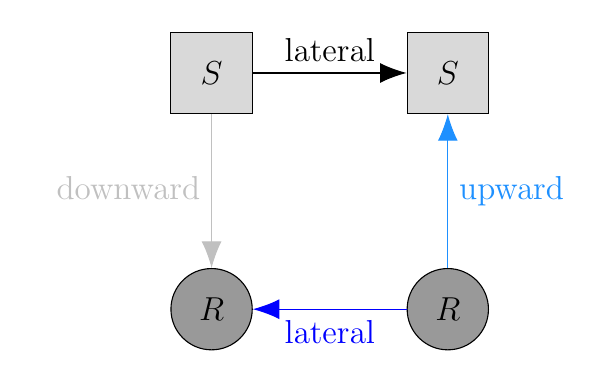
\begin{tikzpicture}[shorten >=0pt,node distance=3cm and 3cm,on grid,auto] 
    \large
\node[state] (s1) [align=center,fill=gray!30,rectangle] {$S$};
\node[state] (s2) [align=center,fill=gray!30,rectangle, right=of s1] {$S$};
\node[state] (r1) [align=center,fill=gray!80, below=of s1] {$R$};
\node[state] (r2) [align=center,fill=gray!80, right=of r1] {$R$};
\path[-{Latex[scale=2.0]}]
(s1) edge [align=center] node {lateral} (s2)
(s1) edge [left,color=silver] node {\phantom{p}downward} (r1)
(r2) edge [right,color=dodgerblue] node {upward} (s2)
(r2) edge [align=center,color=blue] node {lateral} (r1)
;
\end{tikzpicture}
\end{document}